%%%%%%%%%%%%%%%%%%%%%%%%%%%%%%%%%%%%%%%%%
% Beamer Presentation
% LaTeX Template
% Version 1.0 (10/11/12)
%
% This template has been downloaded from:
% http://www.LaTeXTemplates.com
%
% License:
% CC BY-NC-SA 3.0 (http://creativecommons.org/licenses/by-nc-sa/3.0/)
%
%%%%%%%%%%%%%%%%%%%%%%%%%%%%%%%%%%%%%%%%%

%----------------------------------------------------------------------------------------
%	PACKAGES AND THEMES
%----------------------------------------------------------------------------------------

\documentclass{beamer}

\mode<presentation> {

% The Beamer class comes with a number of default slide themes
% which change the colors and layouts of slides. Below this is a list
% of all the themes, uncomment each in turn to see what they look like.

%\usetheme{default}
%\usetheme{AnnArbor}
%\usetheme{Antibes}
%\usetheme{Bergen}
%\usetheme{Berkeley}
%\usetheme{Berlin}
%\usetheme{Boadilla}
%\usetheme{CambridgeUS}
%\usetheme{Copenhagen}
%\usetheme{Darmstadt}
%\usetheme{Dresden}
%\usetheme{Frankfurt}
%\usetheme{Goettingen}
%\usetheme{Hannover}
%\usetheme{Ilmenau}
%\usetheme{JuanLesPins}
%\usetheme{Luebeck}
\usetheme{Madrid}
%\usetheme{Malmoe}
%\usetheme{Marburg}
%\usetheme{Montpellier}
%\usetheme{PaloAlto}
%\usetheme{Pittsburgh}
%\usetheme{Rochester}
%\usetheme{Singapore}
%\usetheme{Szeged}
%\usetheme{Warsaw}

% As well as themes, the Beamer class has a number of color themes
% for any slide theme. Uncomment each of these in turn to see how it
% changes the colors of your current slide theme.

%\usecolortheme{albatross}
%\usecolortheme{beaver}
%\usecolortheme{beetle}
%\usecolortheme{crane}
%\usecolortheme{dolphin}
%\usecolortheme{dove}
%\usecolortheme{fly}
%\usecolortheme{lily}
%\usecolortheme{orchid}
%\usecolortheme{rose}
%\usecolortheme{seagull}
%\usecolortheme{seahorse}
%\usecolortheme{whale}
%\usecolortheme{wolverine}

%\setbeamertemplate{footline} % To remove the footer line in all slides uncomment this line
%\setbeamertemplate{footline}[page number] % To replace the footer line in all slides with a simple slide count uncomment this line

%\setbeamertemplate{navigation symbols}{} % To remove the navigation symbols from the bottom of all slides uncomment this line
}

\usepackage{graphicx} % Allows including images
\usepackage{booktabs} % Allows the use of \toprule, \midrule and \bottomrule in tables

%----------------------------------------------------------------------------------------
%	TITLE PAGE
%----------------------------------------------------------------------------------------

\title[Midterm report]{Apply machine learning to Performance trend analysis} % The short title appears at the bottom of every slide, the full title is only on the title page

\author{Araya Eamrurksiri} % Your name
\institute[] % Your institution as it will appear on the bottom of every slide, may be shorthand to save space
{
 \\ % Your institution for the title page
\medskip
\textit{} % Your email address
}
\date{March 28, 2017} % Date, can be changed to a custom date

\begin{document}

\begin{frame}
\titlepage % Print the title page as the first slide
\end{frame}

\begin{frame}
\frametitle{Overview} % Table of contents slide, comment this block out to remove it
\tableofcontents % Throughout your presentation, if you choose to use \section{} and \subsection{} commands, these will automatically be printed on this slide as an overview of your presentation
\end{frame}

%----------------------------------------------------------------------------------------
%	PRESENTATION SLIDES
%----------------------------------------------------------------------------------------
%\begin{frame}
%\frametitle{Introduction}
%Sometimes a time series is consists of observations generated by different behavior at different times. It would act switching back and forth between a several of distinct states, or regimes.
%\end{frame}

%------------------------------------------------
\section{Recall: Thesis objectives}
\begin{frame}
\frametitle{Objectives}
\begin{itemize}
	\item Detect the state of the \texttt{CPU utilization} (degrading, improving or steady state)
	\item Detect whether there is any change in the test environment that effects the \texttt{CPU utilization}
\end{itemize}
\end{frame}

%------------------------------------------------

\section{Markov switching model} % Sections can be created in order to organize your presentation into discrete blocks, all sections and subsections are automatically printed in the table of contents as an overview of the talk
\begin{frame}
	\frametitle{Markov switching model, \cite{p1}}
	\begin{itemize}
		\item A technique uses for describing the evolution of the process at different period of time
		\item Model involves multiple structures that can characterize the time series behaviors in different states
		\item The switching mechanism between the states is assumed to be an unobserved Markov chain - \footnotesize{a stochastic process which contains the probability of transition from one state to any other state}
	\end{itemize}

\begin{figure}
	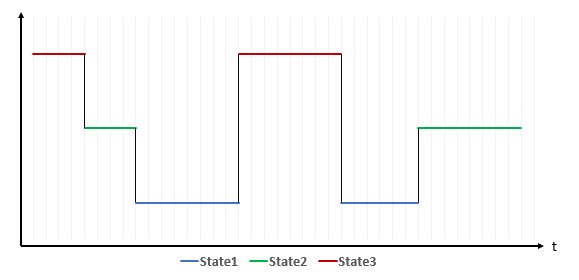
\includegraphics[width=0.5\linewidth]{graph3}
	\caption{regime shift between states}
\end{figure}

\end{frame}

%------------------------------------------------
\begin{frame}
\frametitle{Markov switching model, \cite{p1}}
Assuming that $S_{t}$ denote an unobservable state variable

$$y_{t} = {X_{t}}'\beta_{S_{t}} + \varepsilon_{t}, \quad \varepsilon_{t} \sim N(0,\sigma^{2}_{S_{t}})$$

$y_{t}$ is the observed value of time series at time $t$ 

$X_{t}$ are the predictor variables of time series at time $t$ 

$\beta_{S_{t}}$ are the coefficients in state $S_{t}$, where $S_{t}=1,2,...,k$


\begin{figure}
	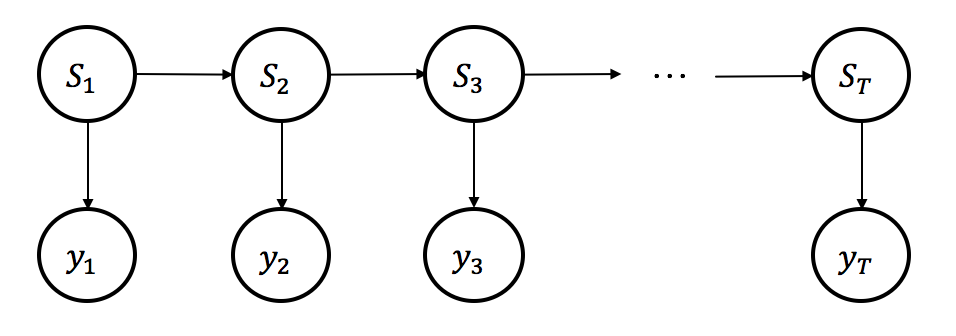
\includegraphics[width=0.5\linewidth]{msm}
	\caption{Model structure}
\end{figure}

\end{frame}

%------------------------------------------------
\begin{frame}
\frametitle{Markov switching model}

Given dataset,

$$y_{t} = {X_{t}}'\beta_{S_{t}} + \varepsilon_{t}, \quad \varepsilon_{t} \sim N(0,\sigma^{2}_{S_{t}})$$

\begin{itemize}
	\item $y_{t}$ is \texttt{CPU utilization}
	\item$X_{t}$ are components which have an impact on the \texttt{CPU utilization}
	\item Assume there are three states ($k=3$): normal, good, bad
\end{itemize}

\begin{figure}
	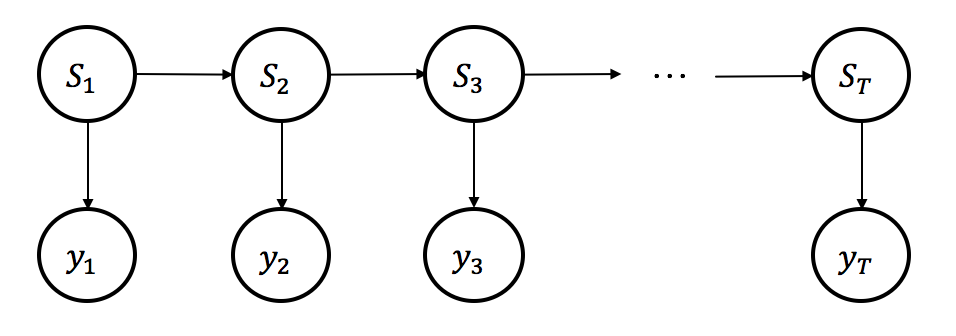
\includegraphics[width=0.5\linewidth]{msm}
	\caption{Model structure}
\end{figure}

\end{frame}

%------------------------------------------------
\subsection{Markov switching autoregressive model} % A subsection can be created just before a set of slides with a common theme to further break down your presentation into chunks

\begin{frame}
\frametitle{Markov switching autoregressive model}

Autoregressive model

$$y_{t} = c + \sum_{i=1}^{p}\phi_{p}y_{t-i} + \varepsilon_{t}$$

where $c$ is constant, $\phi_{p}$ are parameters and $\varepsilon_{t}$ is white noise

\begin{figure}
	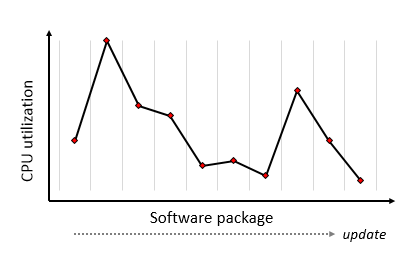
\includegraphics[width=0.6\linewidth]{inde}
\end{figure}
\end{frame}

%------------------------------------------------
\begin{frame}
\frametitle{Markov switching autoregressive model}
The observation are drawn from the first order autoregressive model, AR(1).
%it depends on the past observation and the current state

$$y_{t} = {X_{t}}' \beta_{S_{t}} + \phi_{1,S_{t}} y_{t-1} + \varepsilon_{t}$$

\begin{figure}
	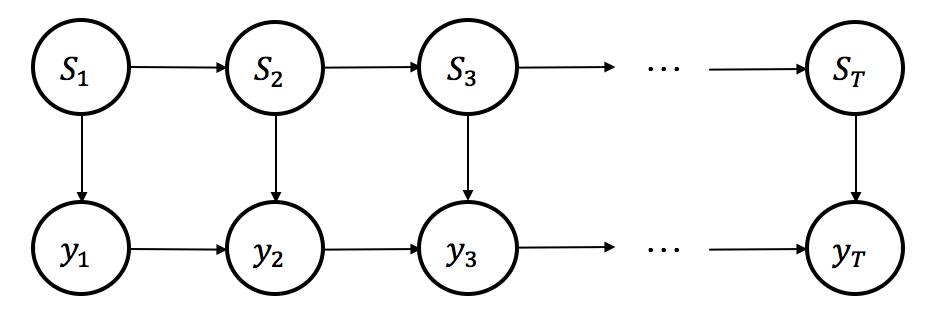
\includegraphics[width=0.5\linewidth]{msm-ar}
	\caption{Model with additional dependencies at observation level}
\end{figure}
\end{frame}

%------------------------------------------------
\section{Model estimation}
\begin{frame}
\frametitle{Model estimation}
Model parameters

$$\theta = (\beta_{S_{t}}, \phi_{1,S_{t}},\sigma^{2}_{S_{t}}, \pi_{S_{t}}, p_{ij})$$

where,

$\pi_{S_{t}}$ is initial probabilities in state $S_{t}$

$p_{ij}$ is transition probabilities, $p_{ij}=P(S_{t}=j|S_{t-1}=i) \quad 1\leqslant i,j\leqslant k $

and $S_{t}$ is non-observable variable

\vspace{5mm}

Model Likelihood

$$L(\theta;y_{t}) = f(y_{t}|\theta) = \sum_{t=1}^{T}\sum_{S_{t}=1}^{k} f(y_{t}|S_{t};\theta)P(S_{t})$$

\end{frame}

%------------------------------------------------
\subsection{E-M algorithm}
\begin{frame}
\frametitle{Model estimation}	
E-M algorithm 
\begin{itemize}
	\item Expectation step: Calculate the expectation of $S_{t}$ given the observation under the current estimated parameters
	\item Maximization step: Obtain new estimates of the parameters by maximizing likelihood 
	\item Repeat until converged
\end{itemize}

\end{frame}

%------------------------------------------------
\section{What has been done?}

\begin{frame}
\frametitle{What has been done?}
One software product $\Rightarrow$ many software packages
	
One software package $\Rightarrow$ many different types of test cases

\vspace{3mm}

Data preprocessing 

\begin{itemize}
	\item Select a test case which has a minimum value of \texttt{CPU utilization} for each software package
	\item Multiple values separated by a tab character are stored together in column $\Rightarrow$ split a tab-separated values to columns
	\item Remove incomplete test cases 
	
\end{itemize}
	
\begin{figure}
	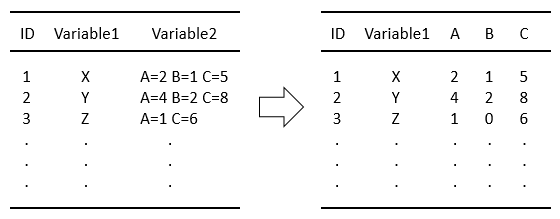
\includegraphics[width=0.55\linewidth]{table4}
	\caption{Data example}
\end{figure}

\end{frame}


%------------------------------------------------
\begin{frame}
\frametitle{What has been done?}
Study and review source code  in the R package in detail
\begin{itemize}
	\item MSwM: An univariate autoregressive Markov switching model for linear and generalized model by using the EM algorithm \cite{p3}
\end{itemize}
\end{frame}

%------------------------------------------------
\begin{frame}
\frametitle{What has been done?}
Implement and modify code in the package
\begin{itemize}
	\item Small typo in the code when computing residual variance
	\item Solve non-invertible Hessian using generalized inverse procedure \cite{p2}
	\item Extension for categorical predictor variables
	\item Deal with NA coefficients
	
	$\Rightarrow$ Mostly occurs when predictor variables are categorical
	
	$\Rightarrow$ Initial coefficients with random subsets
	
	$\Rightarrow$ A single value or incomplete levels of variable
	
	
\end{itemize}
\end{frame}

%------------------------------------------------
\begin{frame}
\frametitle{What has been done?}
Results of fitting Markov switching autoregressive model
\begin{itemize}
	\item Estimated parameters in each state
	\item For each observation,
	
	$\Rightarrow$ State assignment
	
	$\Rightarrow$ Probability assignment in each state
	
	\item Graphs show periods where the observation is in the specific state
\end{itemize}

\end{frame}

%------------------------------------------------
\section{Next step}
\begin{frame}
\frametitle{Next step}
\begin{itemize}
	\item Model selection: Compare several models (e.g., number of states, number of parameters which have switching effects)
	\item State prediction: Find the most probable state for the new observation
	\item Making a state inference
	\item Fit model for other software products

\end{itemize}
\end{frame}

%------------------------------------------------
\begin{frame}
\frametitle{References}
\footnotesize{
	\begin{thebibliography}{99} % Beamer does not support BibTeX so references must be inserted manually as below
		\bibitem[Hamilton, 1989]{p1} James D Hamilton (1989)
		\newblock A new approach to the economic analysis of nonstationary time series and the business cycle
		\newblock \emph{Econometrica: Journal of the Econometric Society}, pages 357-384.
	\end{thebibliography}
	\begin{thebibliography}{99} % Beamer does not support BibTeX so references must be inserted manually as below
		\bibitem[Gill, 2004]{p2} Jeff Gill and Gary King (2004)
		\newblock What to do when your hessian is not invertible:
		Alternatives to model respecification in nonlinear estimation
		\newblock \emph{Sociological
			methods \& research}, 33(1):54-87.
	\end{thebibliography}
	\begin{thebibliography}{99} % Beamer does not support BibTeX so references must be inserted manually as below
		\bibitem[Sanchez-Espigares, 2014]{p3} Josep A. Sanchez-Espigares and Alberto Lopez-Moreno (2014)
		\newblock MSwM: Fitting Markov Switching Models
		\newblock \emph{CRAN R}.
	\end{thebibliography}
}
\end{frame}

\end{document} 